\section{Petri Nets}
A Petri Net is a business process modeling notation, based on some strong mathematical foundations. They offer a formal way 
to represent processes, allowing for rigorous analysis and verification of process properties.
\subsection{Unformal introduction to Petri Nets}
\paragraph{Elements of a Petri Net:}
A Petri Net consists of the following elements:
\begin{itemize}
    \item \textbf{Places}: represent the states or conditions of the system;
    \item \textbf{Transitions}: represent the events that can change the state of the system;
    \item \textbf{Tokens}: represent the presence of a condition or the resources required for a transition to occur;
    \item \textbf{Arcs}: connect places to transitions and transitions to places, indicating the flow of tokens.
\end{itemize}
\begin{figure}[H]
    \centering
    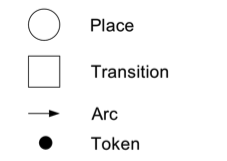
\includegraphics[width=0.3\textwidth]{images/PetriNets/legend.png}
    \caption{Basic Petri Net Structure}
\end{figure}
\paragraph{Syntactic Rules:}
A Petri net can be defined as a \textbf{bipartite directed graph} with two types of nodes: places and transitions. 
The arcs between these nodes indicate the flow of tokens and define the behavior of the system.
\\The \textbf{state} of a Petri net (\textbf{marking}) is represented by the distribution of tokens across its places.
\begin{itemize}
    \item A transition is \textbf{enabled} if all its input places contain the required number of tokens;
    \item When an enabled transition \textbf{fires}, it consumes tokens from its input places and produces tokens in its output places.
\end{itemize}

\subsection{Formal Definition of Petri Nets}
A Petri net is formally defined as a \textbf{triple} \(PN = (P, T, F)\) where:
\begin{itemize}
    \item \(P\) is a finite set of places;
    \item \(T\) is a finite set of transitions;
    \item \(F \subseteq (P \times T) \cup (T \times P)\) is a set of directed arcs (flow relation). They connect places to transitions and transitions to places.
\end{itemize}
Any diagram can be mapped onto such triple and vice versa.
\begin{figure}[H]
    \label{fig:petri_formal}
    \centering
    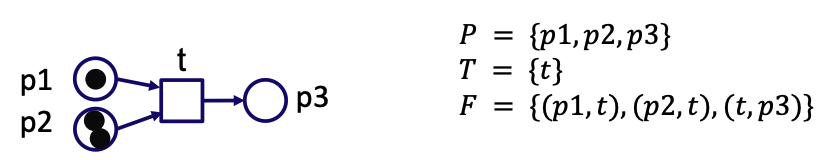
\includegraphics[width=0.7\textwidth]{images/PetriNets/triple.png}
    \caption{Formal Definition of a Petri Net}
\end{figure}
\subsubsection*{Preset and Postset}
For a given transition \(t \in T\):
\begin{itemize}
    \item The \textbf{preset} of \(t\) is the set of places that have arcs leading to \(t\):
    \[\bullet t = \{p \in P | (p, t) \in F\}\]
    \item The \textbf{postset} of \(t\) is the set of places that have arcs leading from \(t\):
    \[t \bullet = \{p \in P | (t, p) \in F\}\]
\end{itemize}
\subsubsection*{Marking}
A \textbf{marking} of a Petri net is a function \(M: P \rightarrow \mathbb{N}\) that assigns to each place $p \in P$ the number of tokens $M(p)$ present in that place.
For example, given the Petri net in the figure \ref{fig:petri_formal}, it's marking can be represented as:
\[M(p1) = 1, M(p2) = 2, M(p3) = 0\]

\subsubsection*{Enabling and Firing}
A transition \(t \in T\) is \textbf{enabled} under a marking \(M\) if for every place \(p \in \bullet t\), \(M(p) > 0\).
In other words, there is at least one token in each of its input places.
\\\\When an enabled transition \(t\) \textbf{fires}, it produces a new marking \(M'\) defined as follows:
\[M'(p) = M(p) - W(p, t) + W(t, p)\]
where \(W(x, y)\) is the weight of the arc from \(x\) to \(y\) (default is 1 if not specified).
This means that firing \(t\) consumes tokens from its input places and produces tokens in its output places.

\subsubsection*{Petri Net System}
A \textbf{Petri net system} is a pair \(S = (PN, M_0)\) where:
\begin{itemize}
    \item \(PN\) is a Petri net \( (P, T, F) \);
    \item \(M_0\) is the initial marking of the Petri net.
\end{itemize}
%# TODO: add petriNet modelling??

\subsection{Mapping Petri Nets to Transition Systems}
To introduce the relationship between Petri nets and transition systems, we first need to define a few concepts.
\paragraph{Case:} a case of a Petri net is a sequence of valid transition firings that starts from the initial marking:
\[ m_0 \xrightarrow{t_1} m_1 \xrightarrow{t_2} m_2 \xrightarrow{t_3} ... \xrightarrow{t_k} m_k \]
where each \(m_i\) is a marking and each \(t_i\) is a transition, $m_0$ is the initial marking.